\documentclass[12pt]{article}

\pagestyle{empty}
\setcounter{secnumdepth}{2}
%----------------------------------------------------------------------------------------
%   Packages and configurations
%----------------------------------------------------------------------------------------
\usepackage[dutch]{babel}
\usepackage{hyperref} %Allow for references
\hypersetup{
    colorlinks,
    citecolor=black,
    filecolor=black,
    linkcolor=black,
    urlcolor=black
} %Set up hyperlink colours.
\newcommand{\sectionbreak}{\clearpage} % Should start every section on its own page
\usepackage{geometry} % Required to change the page size to A4
\geometry{a4paper} % Set the page size to be A4 as opposed to the default US Letter
\usepackage{chngpage}
\usepackage{appendix}
%REMOVE IF HEADER/FOOTER BROKEN
\usepackage{fancyhdr} % Required for custom headers
\usepackage{extramarks} % Required for headers and footers
\usepackage{lastpage} % Required to determine the last page for the footer
%-----------------1
\topmargin=0cm
\oddsidemargin=0cm
\textheight=22.0cm
\textwidth=16cm
\parindent=0cm
\parskip=0.15cm
\topskip=0truecm
\raggedbottom
\abovedisplayskip=3mm
\belowdisplayskip=3mm
\abovedisplayshortskip=0mm
\belowdisplayshortskip=2mm
\normalbaselineskip=12pt
\normalbaselines
\usepackage{listings}
\usepackage[svgnames,table,xcdraw]{xcolor}
\lstset { 
    language=C,
    frame=single,
    escapeinside={\%*}{*)}, 
    breaklines=true,  
    backgroundcolor=\color{black!5},
    basicstyle=\footnotesize,
    commentstyle=\color{mygreen},
    numberstyle=\tiny\color{mygray},
    rulecolor=\color{black},
    keywordstyle=\color{blue},
}
\definecolor{mygreen}{rgb}{0,0.6,0}
\definecolor{mygray}{rgb}{0.5,0.5,0.5}
\definecolor{mymauve}{rgb}{0.58,0,0.82}
\usepackage{wasysym}
\pagestyle{fancy}
\lhead{\textsc{Beckett} \& \textsc{Mathijssen}} % Top left header
\rhead{Opdrachten week 3} % Top center header
\lfoot{
\includegraphics[height=0.8cm]{avans}} % Bottom left footer
\cfoot{} % Bottom center footer
\rfoot{Pagina\ \thepage} % Bottom right footer
\renewcommand\headrulewidth{0.4pt} % Size of the header rule
\renewcommand\footrulewidth{0.4pt} % Size of the footer rule
\usepackage{graphicx} % Required for including pictures

\usepackage{float} % Allows putting an [H] in \begin{figure} to specify the exact location of the figure
\usepackage{wrapfig} % Allows in-line images such as the example fish picture
\usepackage{lipsum} % Used for inserting dummy 'Lorem ipsum' text into the template
\usepackage{pdfpages}
\usepackage[font={footnotesize}]{caption}
\graphicspath{ {../Images/Logos/}{../Images/}{../Images/Week1/} {../Images/Week2/}}
\setlength\parindent{0pt} % Removes all indentation from paragraphs
%\usepackage{showframe}
\newcommand*{\SignatureAndDate}[1]{%
    \par\noindent\makebox[2.5in]{\hrulefill} \hfill\makebox[2.0in]{\hrulefill}%
    \par\noindent\makebox[2.5in][l]{#1}      \hfill\makebox[2.0in][l]{Date}%
}%Signature package
\begin{document}
\begin{titlepage}
\pagenumbering{Roman}
\newcommand{\HRule}{\rule{\linewidth}{0.5mm}} % Defines a new command for the horizontal lines, change thickness here

\center % Center everything on the page


\includegraphics[height=3cm] {avans}\\% Include a department/university logo - this will require the graphicx package
\textsc{\Large Avans Hogeschool Breda}\\[0.5cm] % Major heading such as course name
\textsc{\large Intelligente wireless sensornetwerken }\\[0.5cm] % Minor heading such as course title
\HRule \\[0.4cm]
{ \huge \bfseries Opdrachten week 3	}\\[0.4cm] % Title of your document
\HRule \\[1.5cm]

\begin{minipage}{0.4\textwidth}
\begin{flushleft} \large
\emph{Auteurs:}\\
Guus \textsc{Beckett} \\% Your name 
Joris \textsc{Mathijssen}
\end{flushleft}
\end{minipage}
~
\begin{minipage}{0.4\textwidth}
\begin{flushright} \large
\emph{Docenten:} \\
Diederich \textsc{Kroeske} \\ % Supervisor's Name
Andries \textsc{van Dongen} \\ % Supervisor's Name
\end{flushright}
\end{minipage}\\[4cm]

{\large \today}\\[3cm] % Date, change the \today to a set date if you want to be precise

Versie: 0.2.0

\vfill % Fill the rest of the page with whitespace

\end{titlepage}

\clearpage
% \section*{Voorwoord}
% \addcontentsline{toc}{section}{Voorwoord}

% Guus Beckett \& Jim van Abkoude \\
% \today \\
% Breda
% \newpage
% \section*{Samenvatting}
% \addcontentsline{toc}{section}{Samenvatting}
% \lipsum[0-2]
% \newpage
% \tableofcontents
% \newpage
\pagenumbering{arabic}
\section*{Opdracht 1 a}
\begin{quote}
Doorloop hoofdstuk 2 vanaf bladzijde 40 en voer de opdrachten uit. In dit hoofdstuk gaat het om de kennismaking met AT-commando’s en het realiseren van een point-to-point(P2P) verbinding tussen twee XBee-nodes(Series2)en de kennismaking met AT-commando’s.Een node is de coordinator en de andere een router.
\end{quote}
We hebben de opdrachten van hoofdstuk 2 uitgevoerd. Via de volgende commandos hebben we een chat opgezet tussen 2 Xbees
\begin{lstlisting}
+++ OK

atid 2016

atwr

atcn
\end{lstlisting}
Hier na was het mogelijk om te communiceren via de terminal met de andere Xbee
\newpage
\section*{Opdracht 1b}
\begin{quote}
1a heb je de 64-bits adressen gebruikt van elk van de nodes (source en destination).In een Zigbee netwerk wordt voor de controller ook het (destination)adres 0 gebruikt.
De controller kan aan alle andere nodes bericht sturen door een broadcast met (destination) adres 0xFFFF. Pas dit toe bij drie nodes:een controller en twee routers: Open drie X-CTU applicaties met elk een node: 1 controller en 2 routers. Stel op de routers voor ‘destinationadress’ het adres met waarde 0 in.Controleer dat de communcatie werkt.
\end{quote}
We hebben eerst de verschillende routers en coordinator geprogrameerd. Guus de 2 routers op zijn mac en ik de coordinator op mijn linux. Op de onderstaande manier hebben we het id veranderd en het address aangepast naar 0. Hierna konden de routers met de coordinator spreken en de coordinator met alle routers.
\begin{lstlisting}
+++ OK

atid 4816

atdl 0

atwr

atcn
\end{lstlisting}	
\begin{figure}[h!]
  \centering
      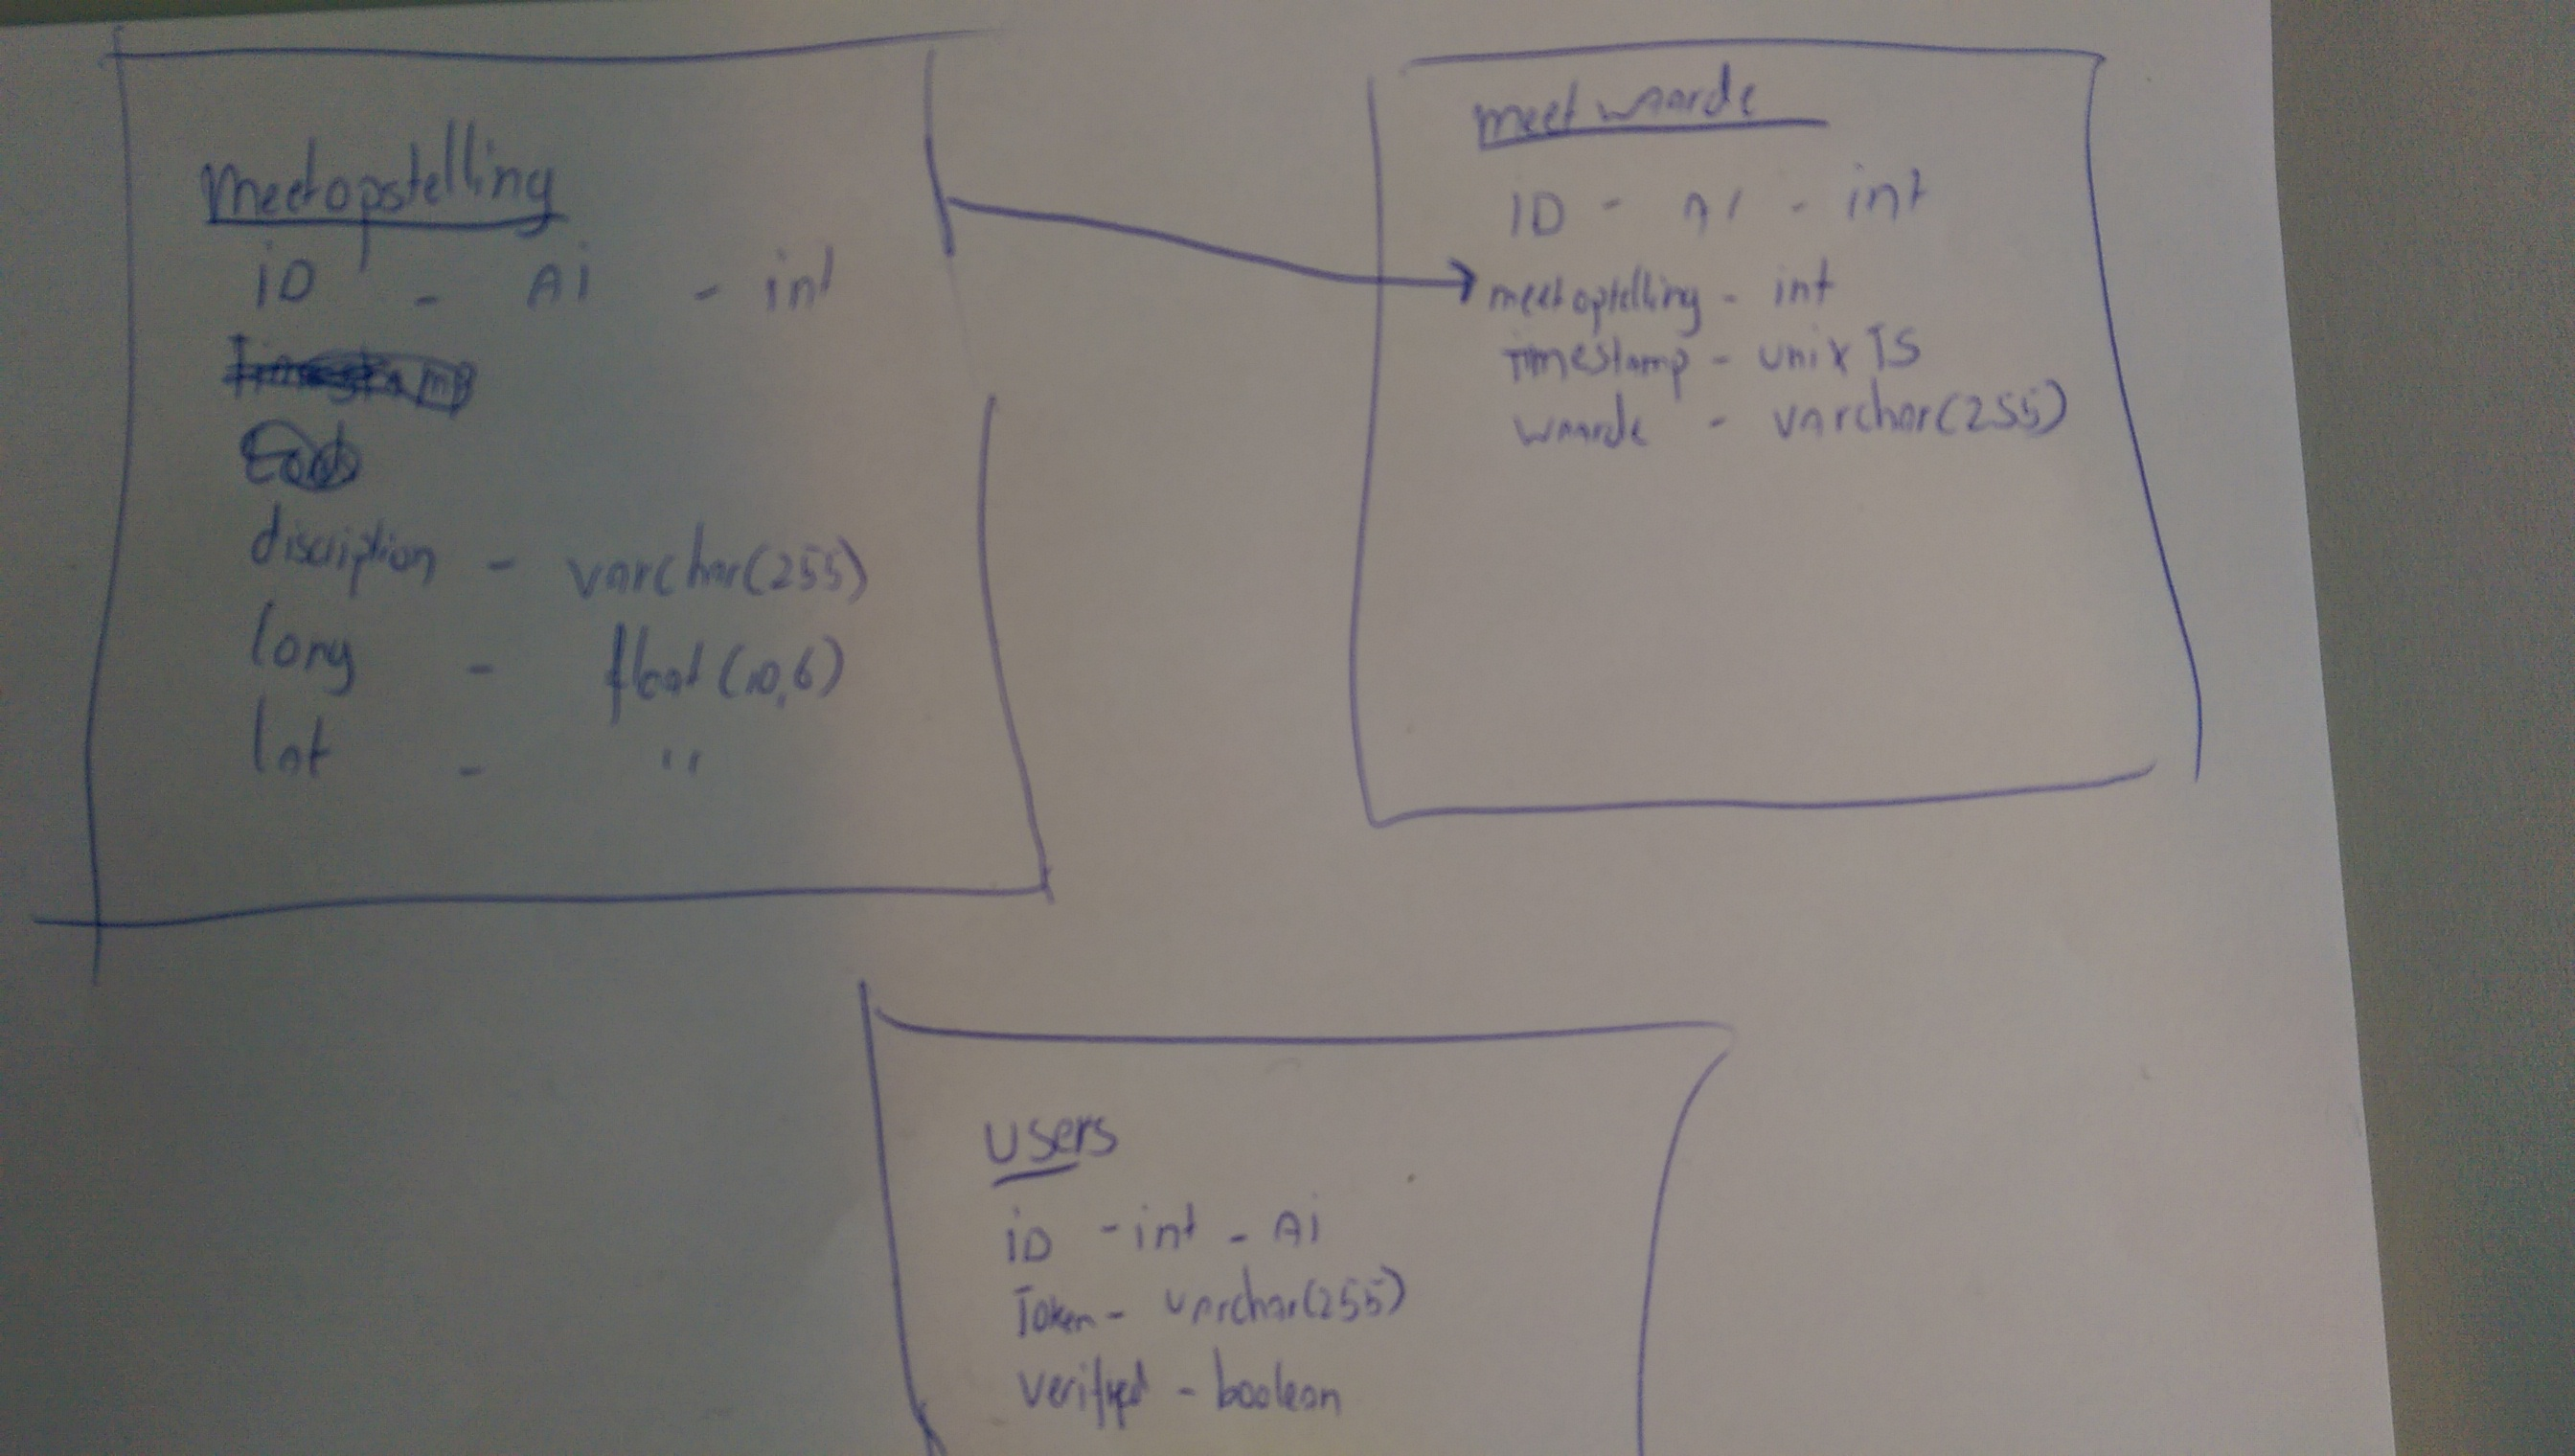
\includegraphics[width=0.8\textwidth]{IMAG0013}
  \caption{Simpele schets van ons database idee}
\end{figure}
\newpage
\end{document}
